\documentclass[border=5pt]{standalone}
\usepackage{tikz}
\usepackage{amsmath}
\begin{document}
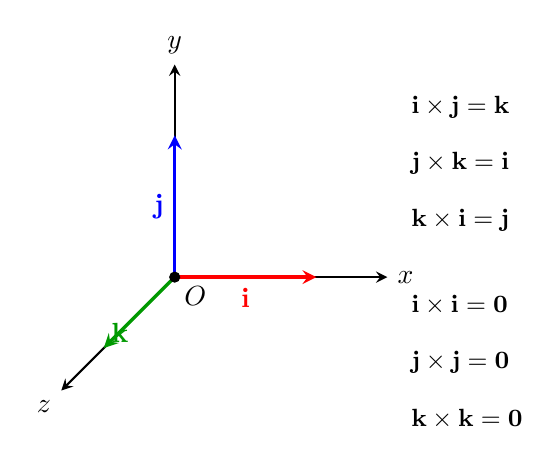
\begin{tikzpicture}[scale=1.8, >=stealth]
  % Right-handed coordinate system with unit vectors

  % Axes
  \draw[->, thick] (0,0) -- (1.5,0) node[right] {$x$};
  \draw[->, thick] (0,0) -- (0,1.5) node[above] {$y$};
  \draw[->, thick] (0,0) -- (-0.8,-0.8) node[below left] {$z$};

  % Unit vectors
  \draw[->, very thick, red] (0,0) -- (1,0) node[midway, below] {$\mathbf{i}$};
  \draw[->, very thick, blue] (0,0) -- (0,1) node[midway, left] {$\mathbf{j}$};
  \draw[->, very thick, green!60!black] (0,0) -- (-0.5,-0.5) node[midway, below left] {$\mathbf{k}$};

  % Labels for cross products
  \node[font=\small, anchor=west] at (1.6, 1.2) {$\mathbf{i}\times\mathbf{j} = \mathbf{k}$};
  \node[font=\small, anchor=west] at (1.6, 0.8) {$\mathbf{j}\times\mathbf{k} = \mathbf{i}$};
  \node[font=\small, anchor=west] at (1.6, 0.4) {$\mathbf{k}\times\mathbf{i} = \mathbf{j}$};

  % Same vector products
  \node[font=\small, anchor=west] at (1.6, -0.2) {$\mathbf{i}\times\mathbf{i} = \mathbf{0}$};
  \node[font=\small, anchor=west] at (1.6, -0.6) {$\mathbf{j}\times\mathbf{j} = \mathbf{0}$};
  \node[font=\small, anchor=west] at (1.6, -1.0) {$\mathbf{k}\times\mathbf{k} = \mathbf{0}$};

  % Origin
  \filldraw[black] (0,0) circle (1pt) node[below right] {$O$};
\end{tikzpicture}
\end{document}
